\documentclass{article}
\usepackage{xcolor}
\usepackage{listings}
\usepackage{pgfgantt}
\definecolor{blue}{HTML}{74BBC9}

\title{Dynamically Scheduled High-Level Synthesis: a Synthesis}
\author{Lana Josipovi\'c, Radhika Ghosal and Paolo Ienne\\ Synthesis by Aur\`ele Barri\`ere}
\date{November 4th, 2018}

\def\todo#1{{\color{red}#1}}

\begin{document}
\maketitle

\section{Introduction}
As more and more companies and datacenters start using FPGAs, the programming paradigms should adapt to a broader range of applications.
The main goal of generating circuits for FPGAs is performance, and using parallelism as much as possible is a key to a shorter execution time.

High-level Synthesis (HLS) tools generate circuits for FPGAs, from languages such as C.
As of today, most HLS tools have a static approach to operation scheduling: the exact cycle where each operation will be executed is decided at synthesis time.
Despite rigorous research on these techniques, static scheduling is fundamentally unable to exploit parallelism in some cases.
For instance, when pipelining a loop, each iteration must follow the same schedule, even if the control-flow differs. To this end, static HLS must always assume the worst-case scenario: every branch might be taken and any two memory accesses might be dependent.

Such information (independence of memory access or whether or not a branch is executed) could be retrieved dynamically, at run-time. Using this information could allow more parallelism.
As a result, this paper presents a new strategy for HLS tools: generating dynamically scheduled circuits.
This would mean that the exact schedule is unknown at synthesis-time, allowing different iterations of a loop to be scheduled differently depending on run-time information.
Of course, extracting such information and delaying scheduling implies an overhead in time and an a bigger circuit complexity, but the overall performance should increase whenever static scheduling could not exploit some instruction parallelism.

The end result is a complete methodology to generate dynamically scheduled circuits from C code. The transformation is automatic and has been implemented, tested and compared with traditional static HLS tools and other dynamic scheduling techniques.


\todo{Parallel with VLIW and superscalar. Solution derives from VLIW tecniques? [28,37].
VLIW, and HLS is really successful for regular programs.}

\section{Dynamic Scheduling}
Static scheduling of a loop has to be correct for every possible iteration.
Consider for instance this minimal example:
\begin{lstlisting}
  for(int i=0; i<100: i++) {
    d = A[i] * 2;
    if (d >= 0) { s += d; }
  } 
\end{lstlisting}
Where \texttt{A} is an array which begins with \texttt{[-1, 2, 3, -2]}.
A static schedule must assume that the \texttt{if} will be taken, and thus each iteration must perform a read, a muliplication, a test, and the addition \texttt{s += d}. Iterations are not independent, as one must wait the end of the addition of the previous iteration before executing the next one.
With pipelining, the best static scheduling one can hope is the following:


\begin{figure}[h]
\hspace{-3cm}
%\centering
\begin{ganttchart}[
		x unit=0.7cm,
		y unit chart=0.7cm,
		canvas/.style={draw=none,fill=none}, % remove canvas borders, etc
		vgrid={*1{draw=black!12}},           % vertical gray lines every unit
		inline,                              % draw bars inline
		group/.style={draw=none,fill=none},  % remove group borders, etc
		bar top shift=0.1,                   % give bar 10% padding top/bottom
		bar height=0.8,                      % bar size 80% of vertical space
		y unit title=0.5cm,                  % crop titles a little smaller
		title/.style={draw=none,fill=none},  % remove title borders, etc
		include title in canvas=false        % no vertical grid in title
	]{-1}{21}

	\ganttgroup[inline=false]{$i=1$}{0}{1}
	\ganttbar[bar/.style={fill=yellow}]{\texttt{Read}}{0}{0}
	\ganttbar[bar/.style={fill=blue}]{\texttt{*}}{1}{4} 
        \ganttbar[bar/.style={fill=yellow}]{\texttt{>=}}{5}{5}
        \ganttbar[bar/.style={fill=red}]{\texttt{+}}{6}{9}\\
        
	\ganttgroup[inline=false]{$i=2$}{0}{1}
	\ganttbar[bar/.style={fill=yellow}]{\texttt{Read}}{4}{4}
	\ganttbar[bar/.style={fill=blue}]{\texttt{*}}{5}{8} 
        \ganttbar[bar/.style={fill=yellow}]{\texttt{>=}}{9}{9}
        \ganttbar[bar/.style={fill=blue}]{\texttt{+}}{10}{13}\\

        \ganttgroup[inline=false]{$i=3$}{0}{1}
	\ganttbar[bar/.style={fill=yellow}]{\texttt{Read}}{8}{8}
	\ganttbar[bar/.style={fill=blue}]{\texttt{*}}{9}{12} 
        \ganttbar[bar/.style={fill=yellow}]{\texttt{>=}}{13}{13}
        \ganttbar[bar/.style={fill=blue}]{\texttt{+}}{14}{17}\\

        \ganttgroup[inline=false]{$i=4$}{0}{1}
	\ganttbar[bar/.style={fill=yellow}]{\texttt{Read}}{12}{12}
	\ganttbar[bar/.style={fill=blue}]{\texttt{*}}{13}{16} 
        \ganttbar[bar/.style={fill=yellow}]{\texttt{>=}}{17}{17}
        \ganttbar[bar/.style={fill=red}]{\texttt{+}}{18}{21}


\end{ganttchart}
\caption{Static scheduling with loop pipelining. Red operations are not actually used}
\label{fig:static_schedule}
\end{figure}

We can notice that, even if some of the additions are not used (whenever \texttt{A[i]} is negative), they are still scheduled. This delays the whole schedule, as the second iteration could start only one cycle after the first one if we knew that the first \texttt{if} wasn't taken.

The idea of dynamic scheduling is to achieve the following one:
\begin{figure}[h]
\hspace{-3cm}
%\centering
\begin{ganttchart}[
		x unit=0.7cm,
		y unit chart=0.7cm,
		canvas/.style={draw=none,fill=none}, % remove canvas borders, etc
		vgrid={*1{draw=black!12}},           % vertical gray lines every unit
		inline,                              % draw bars inline
		group/.style={draw=none,fill=none},  % remove group borders, etc
		bar top shift=0.1,                   % give bar 10% padding top/bottom
		bar height=0.8,                      % bar size 80% of vertical space
		y unit title=0.5cm,                  % crop titles a little smaller
		title/.style={draw=none,fill=none},  % remove title borders, etc
		include title in canvas=false        % no vertical grid in title
	]{-1}{21}

	\ganttgroup[inline=false]{$i=1$}{0}{1}
	\ganttbar[bar/.style={fill=yellow}]{\texttt{Read}}{0}{0}
	\ganttbar[bar/.style={fill=blue}]{\texttt{*}}{1}{4} 
        \ganttbar[bar/.style={fill=yellow}]{\texttt{>=}}{5}{5}\\
        %\ganttbar[bar/.style={fill=red}]{\texttt{+}}{6}{9}\\
        
	\ganttgroup[inline=false]{$i=2$}{0}{1}
	\ganttbar[bar/.style={fill=yellow}]{\texttt{Read}}{1}{1}
	\ganttbar[bar/.style={fill=blue}]{\texttt{*}}{2}{5} 
        \ganttbar[bar/.style={fill=yellow}]{\texttt{>=}}{6}{6}
        \ganttbar[bar/.style={fill=blue}]{\texttt{+}}{7}{10}\\

        \ganttgroup[inline=false]{$i=3$}{0}{1}
	\ganttbar[bar/.style={fill=yellow}]{\texttt{Read}}{2}{2}
	\ganttbar[bar/.style={fill=blue}]{\texttt{*}}{3}{6} 
        \ganttbar[bar/.style={fill=yellow}]{\texttt{>=}}{7}{7}
        \ganttbar[bar/.style={fill=blue}]{\texttt{+}}{11}{14}\\

        \ganttgroup[inline=false]{$i=4$}{0}{1}
	\ganttbar[bar/.style={fill=yellow}]{\texttt{Read}}{3}{3}
	\ganttbar[bar/.style={fill=blue}]{\texttt{*}}{4}{7} 
        \ganttbar[bar/.style={fill=yellow}]{\texttt{>=}}{8}{8}
        %\ganttbar[bar/.style={fill=red}]{\texttt{+}}{18}{21}


\end{ganttchart}
\caption{Dynamic Scheduling}
\label{fig:dynamic_schedule}
\end{figure}

Better instruction parallelism is achieved. The idea to obtain this schedule is to build a circuit that will execute operations as soon as possible (as soon as its inputs are ready). This way, unused operations won't be scheduled (we don't see any red blocks in figure ?). The authors suggest using Elastic Circuits.

\section{Elastic Circuits}

% Cortadella's paper
In [?], Cortadella et al define \textit{Elastic Circuits}, a new scheme for latency-insensitive designs.
Its primary motivation is to create a solution for circuits that might deal with variable delays, for modularity or scalability purposes for instance.
Indeed, if the delay between two connected functional units is not known, then we need to enforce synchronous behaviour: the receiver should wait until the data produced by the sender has been computed, and the sender should wait until the receiver is ready to accept it.
These new circuits implement the SELF protocol, where each unit is equipped with a \textit{Valid} and a \textit{Stop} Signal. When the sender's valid signal is true (meaning that its stored data is valid), and the receiver's stop signal is false (meaning that it can accept new data), then a data transfer occurs. Otherwise, the transfer is delayed. These signals are computed dynamically, and the protocol adds only a small overhead. The result is a circuit that enforces synchronicity, can be obtained automatically and proved to be correct by construction. Elastic ciruits are latency-insisitive, synchronous and adapted for FPGAs.

Inspired by this definition, and [?], which brought elastic circuits to CGRAs, the authors suggest that using elastic circuits woul allow for a dynamic schedule in High-Level Synhesis.
Such components include classical structure simply augmented with the appropriate handshake signals. For instance elastic buffers, elastic FIFOs, elastic Select (multiplexer). As the handshake signals act as tokens in Petri nets, one also needs more components, such as elastic forks that duplicate tokens or elastic joins. Finally, the remaining elastic blocks deal with control flow: elastic branches and elastic merges.
As an example, we present in Figure ? a simplified elastic circuit for the program of section ?.
\begin{figure}
  \center
  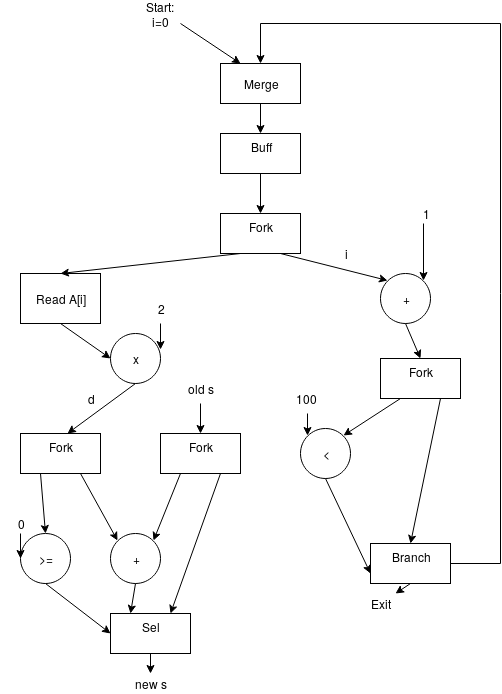
\includegraphics[scale=0.3]{circuit.png}
\end{figure}


\section{Synthesizing Elastic Circuits}
Having chosen elastic circuits, the authors now provide an automatic algortihm to generate them from C code.
They first describe how to transform any \textit{basic block} (part of the code without branching) into an elastic circuits. This transformation is straightforward and resemble many other HLS techniques: any operator is a functional units, and we use elastic forks whenever the result of a node is used several times.
Basic Blocks are themselves connected with elastic merges and elastic branches (one for each variable).
At each block is associated a set \textit{live-in} of variables entering the block, and \textit{live-out} for those used by its successors.
Implementing control flow in elastic circuits require some work to ensure token transfer; one needs to generate (with forks for instance) exactly as many tokens as consumed by successor blocks. To this end, the data propagation information is added to the control-flow graph. The \textit{live-in} and \textit{live-out} sets are modified to ensure that there is no deadlock provided that each cycle has at least one elastic buffer.

As in traditional synchronous circuits, adding elastic buffers can sometimes reduce the critical path's length, without having any effect on the syntheis' correctness. A simple heuristic has been implemented to decide where to add elastic buffers. In the experiments, the heuristic found optimal placements, but this could be an idea for further improvements.

Handling memory accesses is more challenging, as access requests might arrive to memory in any order (the dynamic schedule may be out-of-order).
To make sure that no dependency is \todo{keep going}


\section{Evaluation}
The authors implemented a basic synthesizer following the described techniques.
It uses clang for parsing and SSA generation, one of LLVM's intermediate representations and the LLVM standard optimizations.
The methodology itself is implemented as a transformation from LLVM's IR to an elastic circuit, itself transformed into a VHDL netlist. The end result can be run on a FPGA.

\subsection{Benchmark}
Most programs used in this benchmark are known to present parallelism issues when using static scheduling. This shows the best results one could expect when switching to dynamic scheduling.
The first program \textit{Histogram} goes through an array and increases histogram bars upon finding corresponding values. Statically, we can't determine whether accessing the bars may contain memory dependencies, so we need to assume the worst each time.
The benchmark also includes a \textit{Matrix Power} program, and two loops. The second loop changes the way an operation is performed to show how resource usage in Dynamic HLS can be reduced.
Finally, the benchmark include a \textit{FIR filter}, that is knwon to perform well under static synthesis. This programs allows to estimate the overhead introduced by dynamic scheduling, as no more parallelism can be achieved (every read and write is known to be independent at synthesis-time).

\subsection{Results}
These programs are first compared to Static HLS tools, such as Vivado HLS with pipelin optimization. Comparison fairness is enforced by using the exact same arithmetic units (extracted manually), the same RAMs.
Comparison is done through modelization (with ModelSim).
As no effort has been made yet to optimize the alstic circuits themselves, while static scheduling has benefited from years of study, one could expect to obtain even better results.

Results can be seen on Table ?. One can see significant improvements in execution time for most programs, despite an increase on clock period due to elastic handshake signals.
The results show that the dynamic overhead is negligible compared to the time spared with more parallelism. As expected, the only program where static scheduling performs better is the \textit{FIR filter}, but the difference is minor.
Of course, this execution time improvement requires an added circuit complexity. As a result, elastic circuits are less resource-friendly than static ones. The authors yet argue that the overhead of adding FIFOs would be much less prevalent in bigger programs. Some optimizations could still be done. For instance the second loop is designed to use much less units than the first one.

The new methodology is then compared to other dynamic scheduling techniques.
\todo{describe results}

\section{Conclusion}

\end{document}
